\chapter{Feature Extraction}\label{ch:extraction}
    In this chapter we discuss the different approaches for extracting features from the music. 
    The basis for all our methods are mel spectrograms, which we extract from songs of the Free Music Archive dataset~\cite{FMA}, giving us a decent selection of 8 different genres: Electronic, Experimental, Folk, Pop, Hip-Hop, Instrumental, International, and Rock.

\section{Spectrograms}
    In sound processing, it is difficult to work with the raw signal of any music track.
    Usually the signal is sampled 22050 to 44100 times per second and therefore yields a lot of data points to be processed. 
    Feeding this signal directly to a neural network is inconvenient and single data points don't give a lot of information.
    A way to counter this problem is the short-time Fourier transform. 
    It applies the Fourier transformation on a window of the signal, returning the individual frequencies present at that time frame. 
    Then the window is moved by a given step size, usually smaller than the frame to include some overlap, and the transformation is repeated.
    This results in a spectrogram with information about the magnitude of the individual frequencies and their change over time.\\
    \begin{figure}[!b]
        \centering
        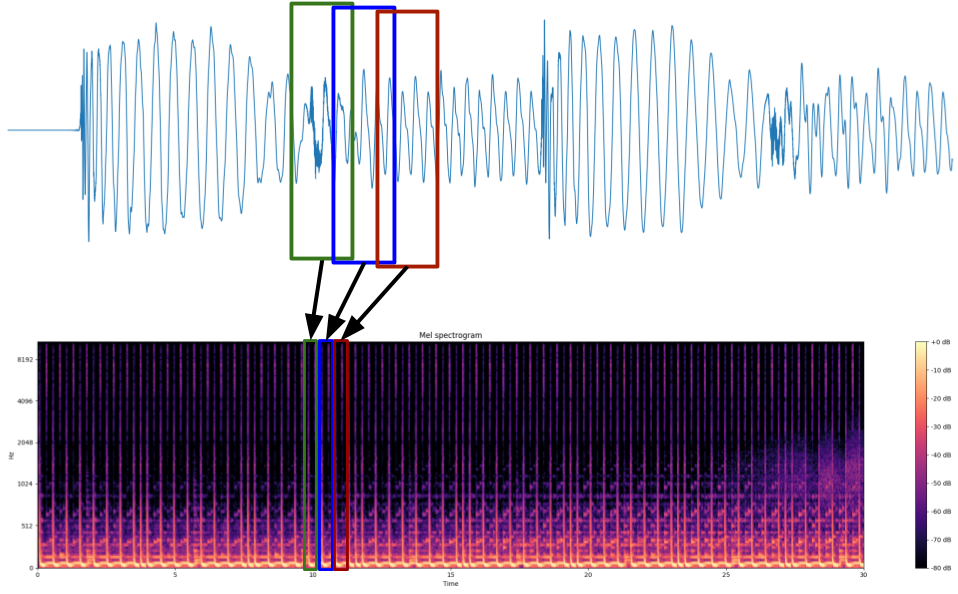
\includegraphics[width=0.8\textwidth]{images/sigToMels.png}
        \caption{The mel spectrogram represents the power of the different frequencies in a frame as they change over time. The powers are mapped to a decibel scale.}
        \label{mel}
    \end{figure}
    \subsection{Mel Spectrograms}
    \indent Mel spectrograms are an extension of the short-time Fourier transform, which map the magnitudes of the frequencies to a logarithmic power scale, to better approximate the human perception of sound.
    For our experiments we sampled the songs with 22050Hz and chose a frame size of 2048 samples for the transformation.
    This corresponds to a window of about 100ms, as bursts of frequencies, which are shorter than this time frame, are perceived less loud by the human ear~\cite{Acoustics}.
    This approximates the human perception of sound for a single time step, eventually giving us correlating images.\\
    To be able to produce 60 fps videos from the music, we chose the step size to be $\lfloor \frac{22050}{60} \rfloor = 367$, also introducing a reasonable amount of overlap, and 128 buckets for the frequencies as the resolution of the spectrum.
    As a last step, we mapped the powers of the mel spectrogram to a decibel scale from -80 to 0, to directly display the sound level of a frequency.\\ 
    \indent Figure~\ref{mel} shows a plot of a mel spectrogram obtained from a 30 second sound snippet of an electronic music track. 
    The recurrent bass line is clearly visible in the visualization, already yielding more visible information about the song than the raw signal.
    These 128-dimensional mel spectrograms are the basis for every of our approaches.

\section{Autoencoder}
    
    \begin{figure}[!t]
    \centering
    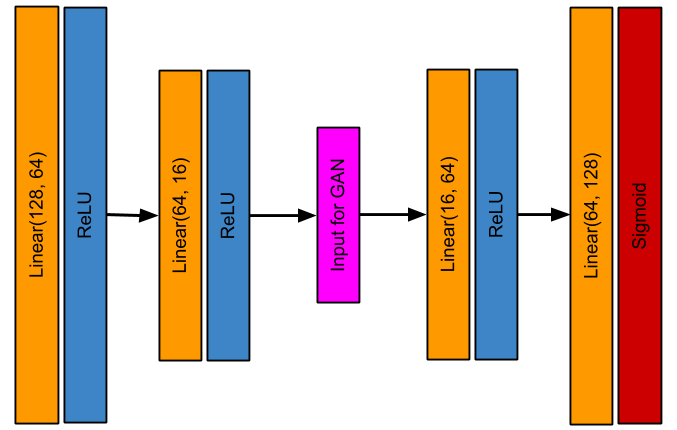
\includegraphics[width=0.75\textwidth]{images/autoencoder}    
    \caption{Architecture of the autoencoder}
    \label{autoencoder}
    \end{figure}
    
    For our second feature method, we trained an autoencoder to reduce the dimensionality of the mel spectrograms down to a much smaller feature space.
    The main idea behind this approach was to use the encoded spectrograms as conditional vectors for the InfoGAN, where the comparatively large original vectors are impractical and would require proportionately larger latent vectors.
    As direct input for a DCGAN, they are somewhat redundant, losing information and complexity compared to the original spectrograms, and should therefore deliver worse results, but we still gave it a try, because why not.
    We will discuss more on this in the next chapters.\\

    \subsection{Architecture}
    \indent Figure~\ref{autoencoder} shows the architecture of the neural network, which we used to encode the vectors. In the first step, we half the dimensionality to 64 dimensions, followed by a rectified linear unit (ReLU).
    The next layer reduces the dimensionality down to the encoded size of 16 dimensions, followed by another ReLU. 
    The resulting vectors after these layers can then serve as potential source of input for a GAN.\\
    \indent The decoding side of the network is symmetric to the encoding side, but ends with the sigmoid function. 
    As the sigmoid function scales the values between 0 and 1, we have to divide the vectors of the mel spectrogram by -80 (they range from -80 to 0) before we put them into the autoencoder, scaling them between 0 and 1 as well. 
    In order to restore the original mel spectrogram, we therefore have to multiply the decoded vectors again with -80.
    As our loss function, we used the MSELoss (mean squared L2 norm) to measure the error between each element of the decoded vector and the original target vector. 
    We trained this setup for 400 epochs.\\
    Figure~\ref{reconstructed} shows a reconstruction of the mel spectrogram from Figure~\ref{mel}, after been passed through the fully trained autoencoder.
    The overall structure of the original spectrogram is clearly maintained, indicating that the autoencoder can compress most of the information into the 16 dimensions of the encoded layer, but still the reconstruction is a bit blurry, smoothes out information and has slightly different magnitudes than the original.
    This result is sufficient for our purposes.

    \begin{figure}
        \centering
        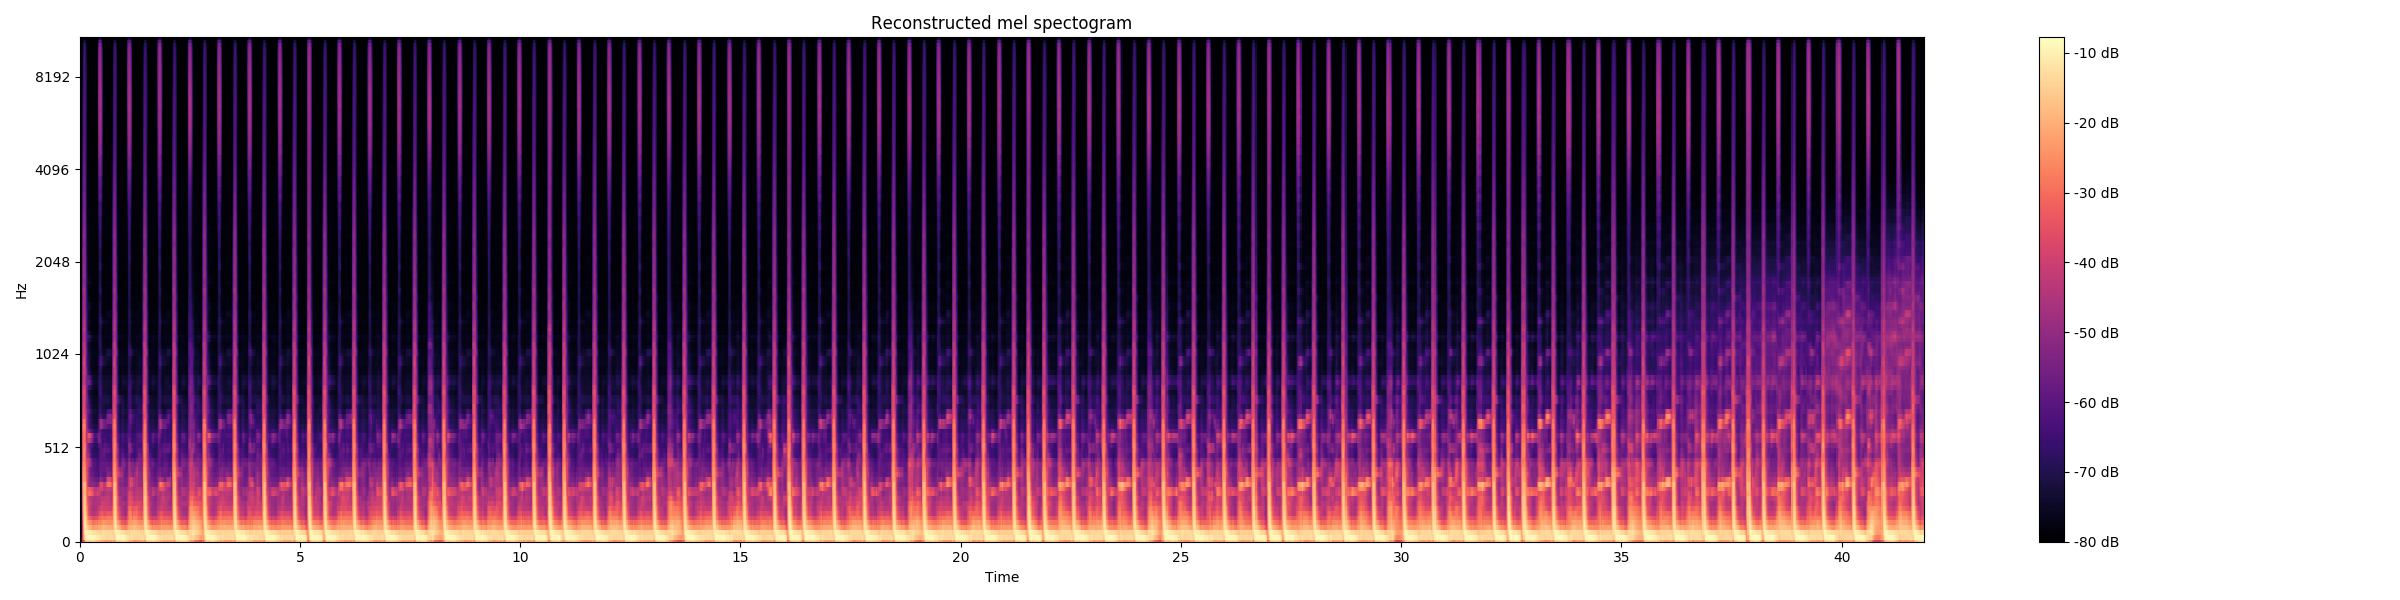
\includegraphics[width=\textwidth, trim=10 0 220 0, clip]{images/recon_spec}
        \caption{Reconstructed mel spectrogram after being encoded and decoded again by our fully trained autoencoder.}
        \label{reconstructed}
    \end{figure}
    
\section{Convolutional Recurrent Neural Network}

    A more sophisticated method was the usage of intermediate features of a convolutional recurrent neural network (CRNN).
    The hope behind this approach was that if we train the network to classify the genre of a song, the convolutional layers at the front will extract features from the mel spectrograms which are specific to the genre, leading to visualizations of the music which correspond not only to the perceived sounds, but also to the respective genre.\\

    \subsection{Architecture}
    In order to keep the temporal coherence of the input vectors throughout the convolutional layers, we had to modify naive realizations of CRNNs.
    Figure~\ref{CRNN} shows our architecture, which we used to classify the 8 different genres of the FMA dataset.
    We input the raw mel spectrograms as a 1D signal with 128 channels and apply a 1-dimensional convolution.
    We use a kernel size of 5 in every convolutional layer and apply a padding of 2 on either side to keep the time steps.
    We have 3 convolutional layers at the front of the network, slowly reducing the feature space down to 32 dimensions, each with ReLUs as their activation function.
    Every layer uses batch normalization and dropout to improve the learning times and stability of the network.
    With this setup, the output of the third convolutional layer has 32 dimensions with genre relevant features and an amount of time steps which is identical to the input, in this case 60 per second.
    This feature map is then used as a potential input to a GAN.\\
    \begin{figure}[t]
        \centering
        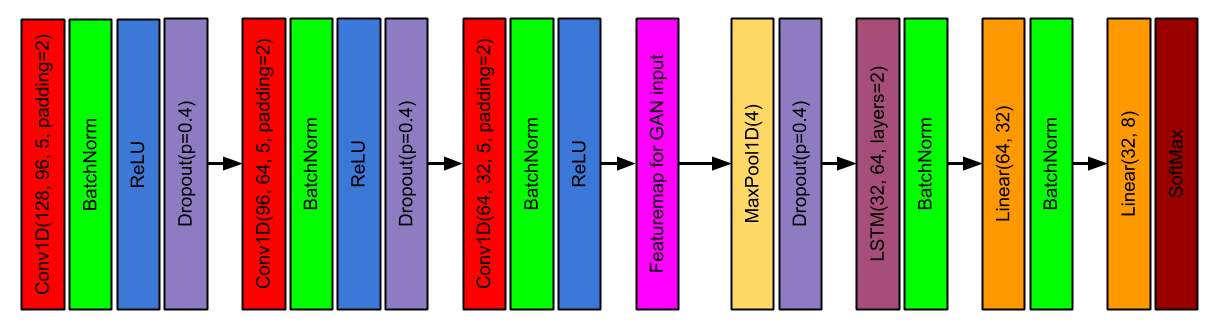
\includegraphics[width=\textwidth]{images/CRNNmodel}
        \caption{Architecture of the convolutional recurrent neural network.}
        \label{CRNN}
    \end{figure}
    Only after the third convolutional layer, we apply a max pooling over 4 time steps, in order to quarter the workload for the following long short-term memory (LSTM) layer with 64 feature dimensions.
    As the convolutional layers only apply their kernel to a relatively small space of the spectrograms, the LSTM layer has to "make sense" out of the sequence of convolutional features.
    A LSTM layer is able to analyze entire sequences of data, being able to remember values over arbitrary time intervals, and therefore fitting perfectly for the classification on the temporal change of the music features.
    This layer collects hidden states over the input time steps, where each hidden state serves as additional input for the succeeding time step, giving it the ability to remember.
    The relevant information is therefore stored in the last hidden state of the LSTM layer, a single 64-dimensional vector, which we can easily give to the following linear layer without the need for a huge amoung of weights.\\
    This linear layer does not have another non-linearity, but this did not seem to influence the performance of the network.
    After that, there is the last linear layer, which connects the 32 neurons of the previous layer to the 8 output neurons, which depict the individual genres.
    We apply a logarithmic softmax function to the output and then use the NLLLoss (negative log likelihood, together with log softmax this is basically the cross entropy loss) to measure the performance of the network during training.\\

    \subsection{Performance Issues}

    \begin{figure}[t]
        \centering
        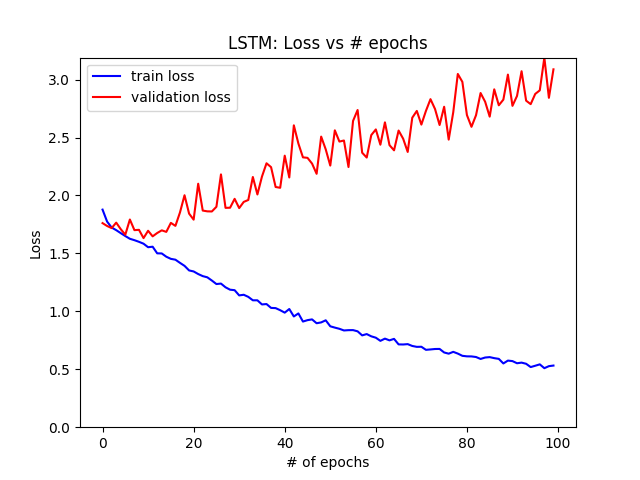
\includegraphics[width=0.49\textwidth]{images/loss}
        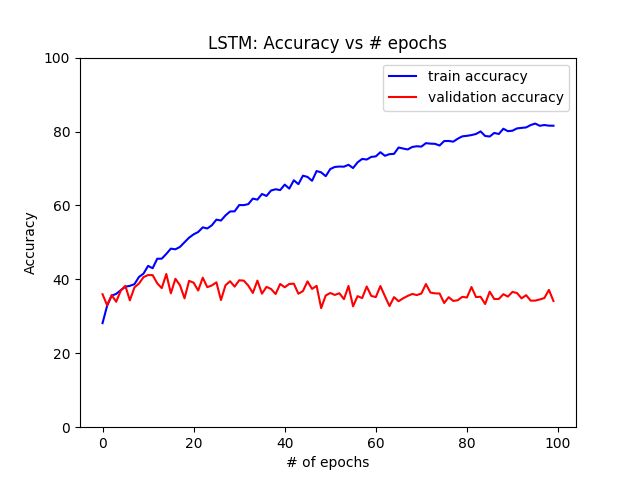
\includegraphics[width=0.49\textwidth]{images/acc}
        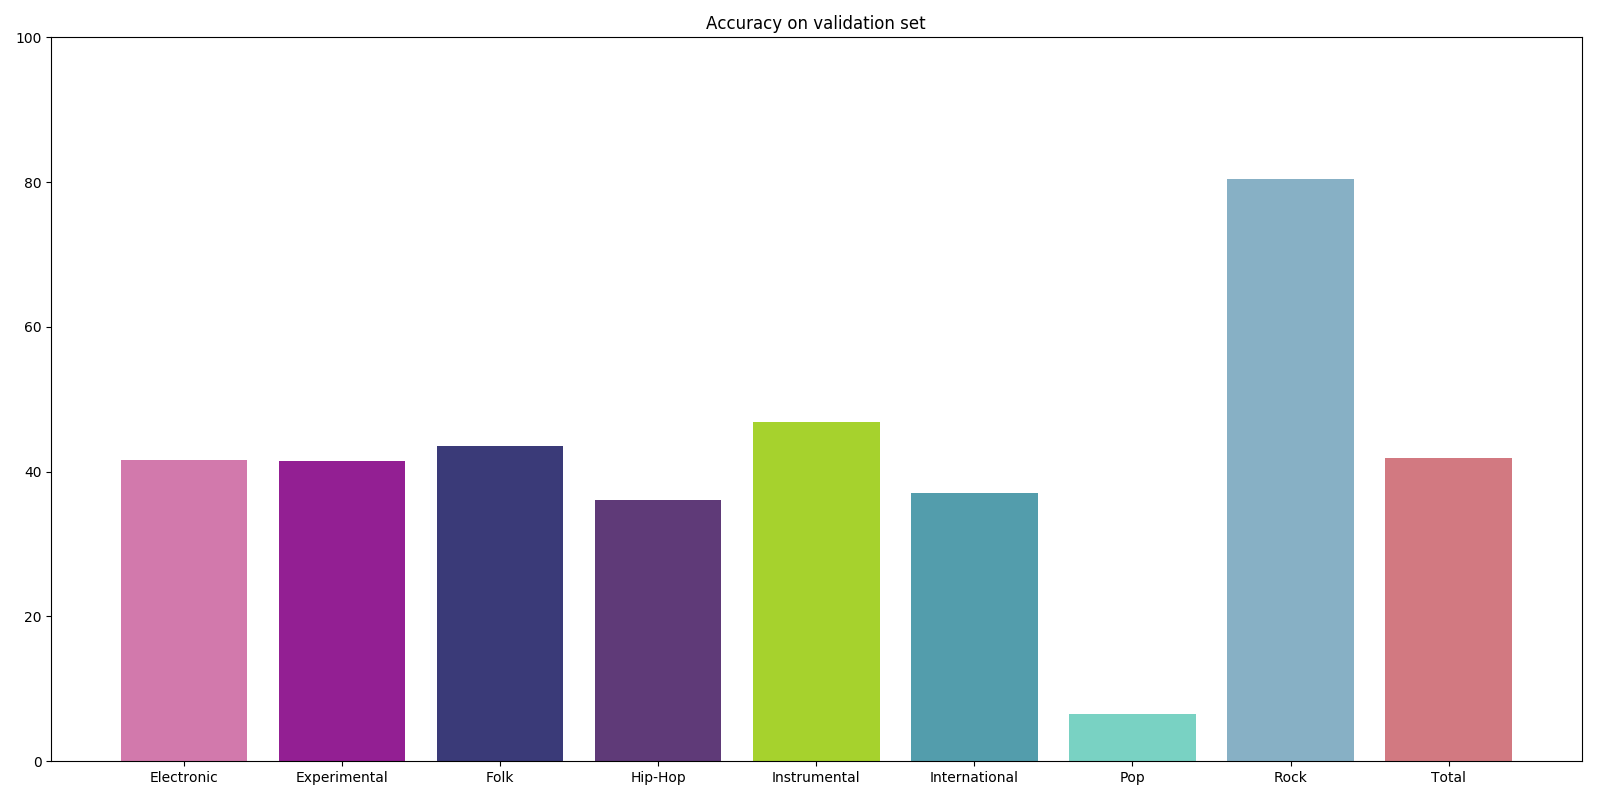
\includegraphics[width=0.91\textwidth]{images/val_acc}
        \caption{Top: loss and accuracy of the CRNN for training and validation over 100 epochs. Bottom: classification accuracy per class of the cherrypicked model at the sweet spot with few overfitting.}
        \label{performance}
    \end{figure}

    Unfortunately, the performance of the network in practice was subpar to levels of comparable networks on this dataset.
    We plotted the loss and accuracy of our CRNN over the first 100 epochs in the top half of Figure~\ref{performance}.
    For the first 15 epochs the network seems to learn some abstraction from the data, performing around 44$\%$ accuracy, but then the validation loss diverges from the training loss and the validation accuracy stagnates.
    Up from this point, the network overfits on the training data, with no real gain on validation.
    This performance is around $20\%$ lower than the top leader board score of the FMA genre recognition challenge~\cite{GenreChallenge} with 63$\%$ and might be due to multiple factors.
    As we had to train a network from scratch to fit our particular needs, the small FMA dataset with its 8000 songs is a relatively small sample size for a deep learning model.
    This leads to the model overfitting very quickly on the training data.
    An approach to counter this could be to split each of the 30 seconds clips into 3 parts of 10 seconds to artificially increase the sample size.
    But in addition, the FMA dataset itself is quite challenging, featuring abstract genres like International or Experimental, as well as Pop, which is just a conglomerate of popular music with no distinct defining sound.
    This has got to be kept in mind when evaluating the model compared to the top scorer with 63$\%$, which also does not sound exceptionally high.\\
    For the generator input, we picked a state of the network right before it starts to overfit on the data, to get the most generic features from the music.
    The bottom image of Figure~\ref{performance} shows our classification accuracies for each of the individual genres of that state.
    Pop is clearly falling off with an accuracy of below 10$\%$, whereas Rock on the other hand is classified correctly around 80$\%$ of the time.
    The other classes gather together at around 40$\%$ with slight differences.
    This introduces some problems for the generator, as the feature space is not well defined and yields ambiguities.
    We tried to gain higher accuracies by reproducing state of the art implementations of CRNNs, but to no avail, we always ended up at similar performance.
    One could argue that the filters of the convolutional layers have problems learning a decent set of weights, as the small step size of the mel spectrograms produce a lot of similar vectors.
    This can lead to plateaus with little change between the time steps, throwing off the filter as it convolves over the input.
    This also might be emphasized by the missing max pooling layers inbetween the convolutions, but our experiments with more reasonable step sizes and max pooling also ended up in similar performance ranges.
    We therefore may have made a mistake somewhere in our system, which we cannot pin down at the moment.
    We still proceeded with the dirty feature map and try to train a generator on the distribution produced by the network. This leads us to our generative adverserial networks.